%%%%%%%%%%%%%%%%%%%%%%%%%%%%%%%%%%%%%%%%%%%%%%%%%%%%%%%%%%%%%%%%%%%%%%%%%%%%%%%%%%%%%%%%%%%%%%%%%%%
% CEI (Centro Espacial ITA) LaTeX Template - Technical Memo
% Based on NASA LaTeX Docs - Configured for Overleaf compilation
%
% AVAILABLE TEMPLATES:
% - template=tech-memo         (Technical Memo - shorter documents)
% - template=tech-report       (Technical Report - longer documents with more sections)
% - template=aiaa-conference   (AIAA Conference Paper)
% - template=aiaa-journal      (AIAA Journal Article)
%%%%%%%%%%%%%%%%%%%%%%%%%%%%%%%%%%%%%%%%%%%%%%%%%%%%%%%%%%%%%%%%%%%%%%%%%%%%%%%%%%%%%%%%%%%%%%%%%%%

\documentclass[template=tech-memo]{nasa-latex-docs}

%%%%%%%%%%%%%%%%%%%%%%%%%%%%%%%%%%%%%%%%%%%%%%%%%%%%%%%%%%%%%%%%%%%%%%%%%%%%%%%%%%%%%%%%%%%%%%%%%%%
% SECTION: Document Parameters - Customize these for your document
%%%%%%%%%%%%%%%%%%%%%%%%%%%%%%%%%%%%%%%%%%%%%%%%%%%%%%%%%%%%%%%%%%%%%%%%%%%%%%%%%%%%%%%%%%%%%%%%%%%

% Document identification
\docTitle[Sample Technical Memo Title]
\docNumber[TM-2024-001]
\docDate[\today]
\docTypeTitle[CEI]

% Header and footer
\docHeader[SAMPLE TECHNICAL MEMO]
\docFooter[]

% Author information
\docAuthor[1]{John Doe}{Engineer}{Engineering Division}{Centro Espacial ITA, São José dos Campos}

% Approver information (optional - leave empty to hide approver section)
% To add an approver, uncomment and fill in:
% \docApprover[1]{Jane Smith}{Manager}{Engineering Division}{Centro Espacial ITA, São José dos Campos}
% To explicitly hide approver section:
\docApprover[1]{}{}{}{}

% Signature information (set to true when ready to sign)
\docSigned[false]
\docSignDate[\today]

% Executive Summary
\docAbstract[
This is a sample executive summary for the technical memo. Replace this text with your actual executive summary that describes the purpose, methodology, and key findings of your technical work.
]

% Logos (CEI and ITA logos are used by default)
% Old NASA logos are kept in images/ folder for reference: Artemis_Logo, NASA_Logo, Orion_Logo
\docLogo[images/CEI_logo]
\docOrgLogo[images/ITA_logo]

% Enable/disable document sections
\docTOC[true]   % Table of Contents - Lists all sections, subsections, etc.
\docLOF[true]   % List of Figures - Lists all figures with captions and page numbers
\docLOT[true]   % List of Tables - Lists all tables with captions and page numbers
\docLOL[false]  % List of Listings - Lists all code listings (if you include code snippets)
\docLOA[false]  % List of Acronyms - Lists all acronyms/abbreviations used in the document

% Export control settings (set to true if applicable)
\docCUI[false]
\docITAR[false]

% Revision log (optional)
% \docRevisionLog[
%    \begin{versionhistory}
%       \vhEntry{1.0}{2024-01-01}{Author Name}{Initial Release}
%    \end{versionhistory}
% ]

%%%%%%%%%%%%%%%%%%%%%%%%%%%%%%%%%%%%%%%%%%%%%%%%%%%%%%%%%%%%%%%%%%%%%%%%%%%%%%%%%%%%%%%%%%%%%%%%%%%
% SECTION: Bibliography
%%%%%%%%%%%%%%%%%%%%%%%%%%%%%%%%%%%%%%%%%%%%%%%%%%%%%%%%%%%%%%%%%%%%%%%%%%%%%%%%%%%%%%%%%%%%%%%%%%%

\addbibresource{bib/main.bib}

%%%%%%%%%%%%%%%%%%%%%%%%%%%%%%%%%%%%%%%%%%%%%%%%%%%%%%%%%%%%%%%%%%%%%%%%%%%%%%%%%%%%%%%%%%%%%%%%%%%
% SECTION: Acronyms (optional)
%%%%%%%%%%%%%%%%%%%%%%%%%%%%%%%%%%%%%%%%%%%%%%%%%%%%%%%%%%%%%%%%%%%%%%%%%%%%%%%%%%%%%%%%%%%%%%%%%%%

% Define acronyms here
% \newacronym{nasa}{NASA}{National Aeronautics and Space Administration}
% \newacronym{cfd}{CFD}{Computational Fluid Dynamics}

%%%%%%%%%%%%%%%%%%%%%%%%%%%%%%%%%%%%%%%%%%%%%%%%%%%%%%%%%%%%%%%%%%%%%%%%%%%%%%%%%%%%%%%%%%%%%%%%%%%
% SECTION: Begin Document
%%%%%%%%%%%%%%%%%%%%%%%%%%%%%%%%%%%%%%%%%%%%%%%%%%%%%%%%%%%%%%%%%%%%%%%%%%%%%%%%%%%%%%%%%%%%%%%%%%%

\begin{document}

%%%%%%%%%%%%%%%%%%%%%%%%%%%%%%%%%%%%%%%%%%%%%%%%%%%%%%%%%%%%%%%%%%%%%%%%%%%%%%%%%%%%%%%%%%%%%%%%%%%
% SECTION: Main Content
%%%%%%%%%%%%%%%%%%%%%%%%%%%%%%%%%%%%%%%%%%%%%%%%%%%%%%%%%%%%%%%%%%%%%%%%%%%%%%%%%%%%%%%%%%%%%%%%%%%

\section{Introduction}

This is a sample technical memo created using the CEI LaTeX template (based on NASA LaTeX Docs\cite{nasa-latex-docs}). Replace this content with your actual technical content.

\section{Background}

Provide background information relevant to your technical work. You can include equations, figures, tables, and references as needed.

\subsection{Methodology}

Describe the methodology used in your technical work.

\section{Results}

Present your results here. \ref{fig:sample_graph} shows a sample figure.

\begin{figure}[H]
   \centering
   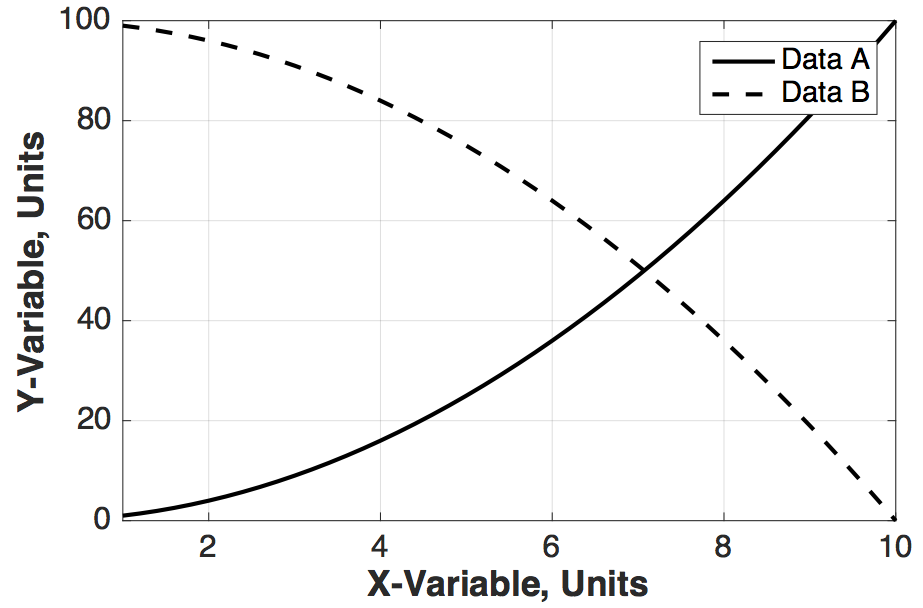
\includegraphics[width=3.5in]{fig/sample_graph}
   \caption{Sample Graph - Replace with your actual figure}
   \label{fig:sample_graph}
\end{figure}

\subsection{Analysis}

Provide analysis of your results.

\section{Conclusions}

Summarize your findings and conclusions.

\section{Recommendations}

Provide any recommendations based on your work.

%%%%%%%%%%%%%%%%%%%%%%%%%%%%%%%%%%%%%%%%%%%%%%%%%%%%%%%%%%%%%%%%%%%%%%%%%%%%%%%%%%%%%%%%%%%%%%%%%%%
% SECTION: Bibliography
%%%%%%%%%%%%%%%%%%%%%%%%%%%%%%%%%%%%%%%%%%%%%%%%%%%%%%%%%%%%%%%%%%%%%%%%%%%%%%%%%%%%%%%%%%%%%%%%%%%

\printbibliography

%%%%%%%%%%%%%%%%%%%%%%%%%%%%%%%%%%%%%%%%%%%%%%%%%%%%%%%%%%%%%%%%%%%%%%%%%%%%%%%%%%%%%%%%%%%%%%%%%%%
% SECTION: Appendices (optional)
%%%%%%%%%%%%%%%%%%%%%%%%%%%%%%%%%%%%%%%%%%%%%%%%%%%%%%%%%%%%%%%%%%%%%%%%%%%%%%%%%%%%%%%%%%%%%%%%%%%

% \begin{appendices}
% 
% \section{Additional Data}
% 
% Include any additional data or supporting information here.
% 
% \end{appendices}

\end{document}
